\documentclass[a4paper,11pt]{scrartcl}
\usepackage[utf8]{inputenc}
\usepackage[english]{babel}
\usepackage{tikz}
\usepackage{amsmath}
\usepackage{dsfont}

\title{Summary: Numerical Simulation of Fluids}

\author{Jan H\"onig \\ \texttt{hrominium@gmail.com}}


\date{\today}


\usetikzlibrary{calc,trees,positioning,arrows,chains,shapes.geometric,%
    decorations.pathreplacing,decorations.pathmorphing,shapes,%
    matrix,shapes.symbols}

\tikzset{
>=stealth',
  punktchain/.style={
    rectangle, 
    rounded corners, 
     fill=black!10,
    draw=black, very thick,
    text width=10em, 
    minimum height=3em, 
    text centered, 
    on chain},
  line/.style={draw, thick, <-},
  element/.style={
    tape,
    top color=white,
    bottom color=blue!50!black!60!,
    minimum width=8em,
    draw=blue!40!black!90, very thick,
    text width=10em, 
    minimum height=3.5em, 
    text centered, 
    on chain},
  every join/.style={->, thick,shorten >=1pt},
  decoration={brace},
  tuborg/.style={decorate},
  tubnode/.style={midway, right=2pt},
}
\begin{document}

\maketitle

%\tableofcontents
%\newpage

\section{Introduction}
How to uncover laws of nature?
\begin{itemize}
	\item practical $\rightarrow$ observation of experiments
	\item theoretical $\rightarrow$ relations ship between mathematical quantities
	\item[!] often experiments impossible (nuclear reactor, oil sill, too long, too short, where to measure) and mathematical equations too complex (only simplified models)
	\item[$\rightarrow$] numerical simulation: combines both aproaches, see Figure~\ref{fig:simproc}
\end{itemize}

\subsection{Simulation Procedure}

\begin{figure}
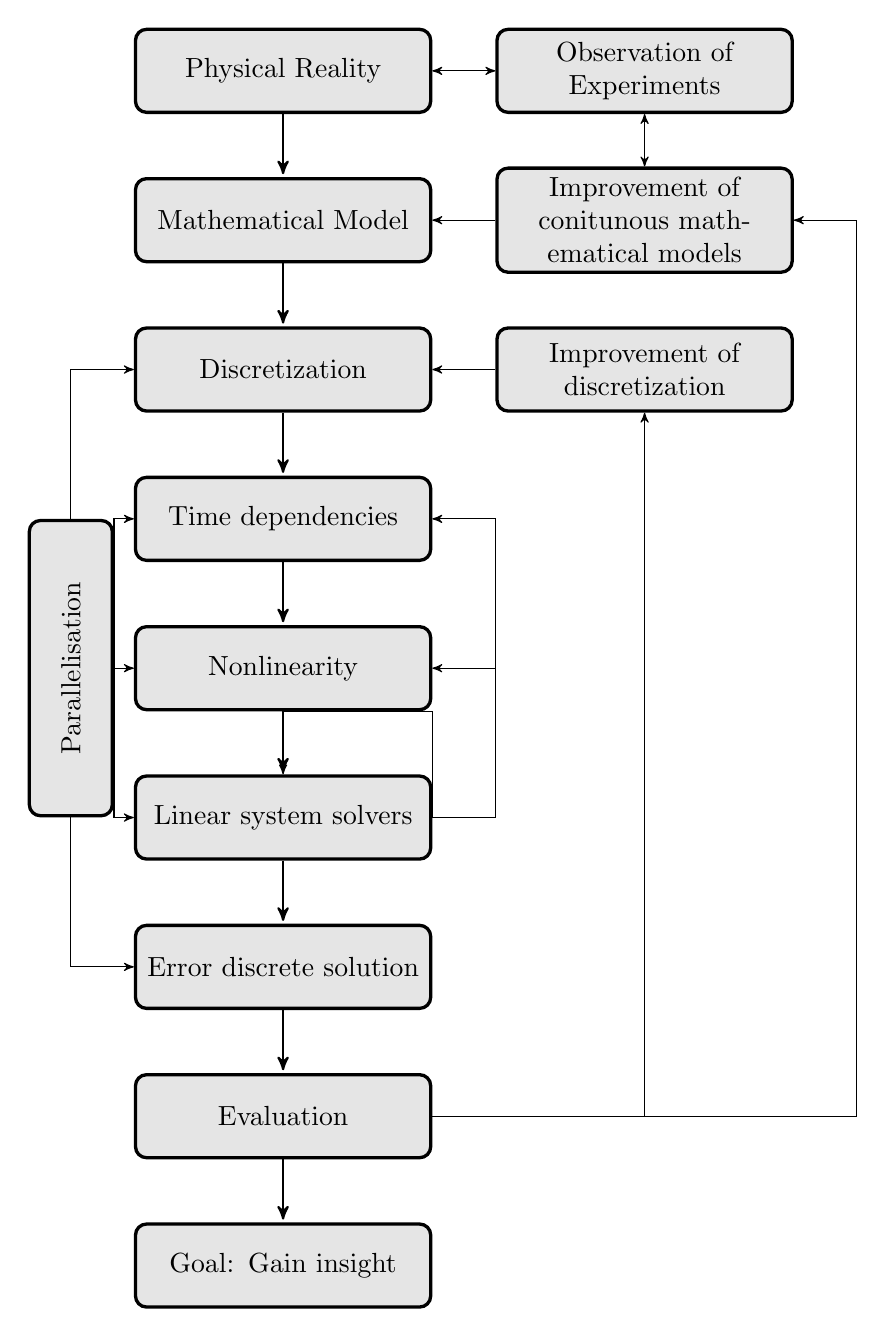
\begin{tikzpicture}
  [node distance=.8cm,
  start chain=going below,]
    \node[punktchain, join] (phys) {Physical Reality};
    \node[punktchain, join] (math)      {Mathematical Model};
    \node[punktchain, join] (discr)      {Discretization};
    \node[punktchain, join] (time-dept) {Time dependencies};
    \node[punktchain, join] (nonlin) {Nonlinearity};
  	\node[punktchain, join] (lin) {Linear system solvers};
    \node[punktchain, join] (error) {Error discrete solution};
    \node[punktchain, join] (eval) {Evaluation};
    \node[punktchain, join] (goal) {Goal: Gain insight};

    \node [punktchain, right=of phys] (obs) {Observation of Experiments};
	\node [punktchain, right=of math] (improvec) {Improvement of conitunous mathematical models};
    \node [punktchain, right=of discr] (improved) {Improvement of discretization};
    \node [punktchain, left=of time-dept, rotate=90] (parallel) {Parallelisation};
	
	\coordinate[right=of lin] (lin-right);
	\coordinate[right,above=of lin] (lin-top);
    
    \coordinate[right=of nonlin] (nonlin-right);

	\draw[->] (lin.east) |- (lin-top) -| (lin.north);
	\draw[->] (lin.east) -| (nonlin-right) -- (nonlin.east);
	\draw[->] (lin.east) -| (nonlin-right) |- (time-dept.east);

    \draw[->] (eval.east) -| (improved.south);
     
    \draw[->] (parallel.east) |- (discr.west);
    \draw[->] (parallel.south) |- (nonlin.west);
    \draw[->] (parallel.south) |- (time-dept.west);
    \draw[->] (parallel.south) |- (lin.west);
    \draw[->] (parallel.west) |- (error.west);

	\coordinate[right=of improvec] (improvec-coord);
	\draw[->] (eval.east) -| (improvec-coord) -- (improvec);

   	\draw[<->] (obs) -- (improvec);
    \draw[<->] (obs) -- (phys);   		   
 		   
  	\draw[->] (improvec) -- (math);   
   	\draw[->] (improved) -- (discr);
	

  \end{tikzpicture}
  
  \renewcommand{\thefigure}{1.1}
  \caption{Typical procedure in numerical simulation}
  \label{fig:simproc}
  \end{figure}

  
\subsection{Fluids and Flows}

Fluids $\left\{
\begin{tabular}{c}
    gas \\
    liquids
\end{tabular}
\right\}$ are substances that cannot resist shear forces. \\
Examples: Water, Coffee, Air, Stream, Waterfall\\
Engeneering: Flow around a car, flow pipeline. Often the iteration of a flow with a solid body, fluid sturcture interaction, multi-phase flows (gas $\leftrightarrow$ liquid).

\paragraph{Properties of Fluids}
\begin{itemize}
	\item Viscosity
	\begin{itemize}
		\item Frictional forces that act on the fluid
		\item[$\rightarrow$] Without external forces the fluid will come to a rest. The higher the viscosity, the faster it comes to a rest.
		\item Highly viscous (honey) $\rightarrow$ frictional forces are strong
		\item In gases viscous forces small $\rightarrow$ sometimes neglected
		\item[$\rightarrow$] "inviscid flow" in gas dynamics $\rightarrow$ Euler equation
	\end{itemize}
	\item Inertia
	\begin{itemize}
		\item[$\rightarrow$] Reynolds number : $\frac{\text{inertia}}{\text{viscosicty}}$
		\item[$\rightarrow$] high $\rightarrow$ turbulence; low $\rightarrow$ laminar
	\end{itemize}
	\item Compressibility
	\begin{itemize}
		\item Gases at high velocities are compressible
		\item Liquids are nearly incompressible
		\item[$\rightarrow$] Important if temperature changes
	\end{itemize}
\end{itemize}

Boundary layer theory
\begin{itemize}
	\item[$\rightarrow$] close to boundary, velocity is slow $\rightarrow$ viscous forces $\sim$ inertia forces
	\item[$\rightarrow$] away from boundaries, velocity high $\rightarrow$ viscous forces $<$ inertia forces
\end{itemize}
%TODO pictures (2)

\subsection{Numerical Fluid Simulation}
Our goal: Simulate unsteady, incompressible, laminar flow, Navier-Stokes equations\\
\paragraph{History}
\begin{itemize}
	\item[$\rightarrow$] Dictated by compute power
	\item precursors: Crank-Nickelson '47
	\item real start: Harlow-Fromm '65
	\item in this course: "marker-and-cell" (MAC) method, Harlow-Welch '65
	\begin{itemize}
		\item simple
		\item flexible
		\item efficient
	\end{itemize}
	\item Alternatives: Finite elements, Finite Volumes, SIMPLE, QUICK
\end{itemize}

\section{Mathematical description of flows}
\begin{itemize}
	\item laminar
	\item viscious
	\item incompressible
\end{itemize}
\subsection{Mathematical Model}
\begin{itemize}
	\item Spatial domain: $\Omega \subset  \mathds{R}^2$ or $\Omega \subset  \mathds{R}^3$
	\item Time $t \in [0, t_{end}]$
	\item Fluid is characteristic by:
	\begin{itemize}
		\item Velocity: $\vec{u} : \Omega \times [0, t_{end}] \rightarrow \mathds{R}^2$
		\item Pressure: $p : \Omega \times [0, t_{end}] \rightarrow \mathds{R}$
		\item Density: $ \varrho : \Omega \times [0, t_{end}] \rightarrow \mathds{R}$
		\item[$\rightarrow$] Incompressible: $\varrho(\vec{x},t) = \varrho_\infty = \text{const}$
	\end{itemize}
\end{itemize}
Governing equations, a system of partial differential equations (Navier-Stokes eq.) are:

\begin{figure}[h]
	\centering
	\[\frac{\delta \vec{u}}{\delta t} + ( \vec{u} \cdot \text{grad}) \vec{u} + \text{grad} p = \frac{1}{Re} \Delta \vec{u} + \vec{g}\]
	\renewcommand{\thefigure}{2.1.a}
    \caption{Momentum Equation}
	\label{fig:momentum}
\end{figure}
\begin{figure}[h]
	\centering
	\[\text{div} \vec{u} = 0\]
	\renewcommand{\thefigure}{2.1.b}
    \caption{Continuity Equation}
	\label{fig:momentum}
\end{figure}

\begin{itemize}
	\item grad $p := (\frac{\delta p}{\delta x},\frac{\delta p}{\delta y})^T$
	\item div $\vec{u} := \frac{\delta u}{\delta x} + \frac{\delta v}{\delta y}$
	\item $\vec{u} \text{ grad} := \left( \begin{pmatrix}
		u \\
		v
	\end{pmatrix}
	\cdot \begin{pmatrix}
		\frac{\delta}{\delta x} \\
		\frac{\delta}{\delta y}
	\end{pmatrix}\right)
	= (u \cdot \frac{\delta}{\delta x} + v \frac{\delta}{\delta y})$
	\item $(\vec{u} \text{ grad} ) \vec{u} = \left( u \cdot \frac{\delta}{\delta x} + v \frac{\delta}{\delta y}\begin{pmatrix}
		u \\
		v
	\end{pmatrix}\right) = \begin{pmatrix}
		u \frac{\delta u}{\delta x} & v \frac{\delta u}{\delta y}\\
		u \frac{\delta v}{\delta x} & v \frac{\delta v}{\delta y}
	\end{pmatrix}$
	\item $Re \in \mathds{R} \Rightarrow$ Reynolds number
	\item $\vec{g} \in \mathds{R} \Rightarrow$ Body forces (i.e. gravity)
	\item $\vec{x} = \begin{pmatrix}
	x\\
	y
	\end{pmatrix}; \vec{u} = \begin{pmatrix}
	u\\
	v
	\end{pmatrix}; \vec{p} = \begin{pmatrix}
	p_x \\
	p_y
	\end{pmatrix}$
\end{itemize}

\begin{figure}[h]
	\centering
	\[ \frac{\delta u}{\delta t} + \frac{\delta p}{\delta x} = \frac{1}{Re} \left( \frac{\delta^2 u}{\delta x^2} + \frac{\delta^2 u}{\delta y^2}\right) - \frac{\delta (u^2)}{\delta x} - \frac{\delta (uv)}{\delta y} + g_x\]
    \renewcommand{\thefigure}{2.2a}
	\caption{Momentum Equation u}
	\label{fig:momentuma}
\end{figure}
\begin{figure}[h]
	\centering
	\[ \frac{\delta v}{\delta t} + \frac{\delta p}{\delta y} = \frac{1}{Re} \left( \frac{\delta^2 v}{\delta x^2} + \frac{\delta^2 v}{\delta y^2}\right) - \frac{\delta (uv)}{\delta x} - \frac{\delta (v^2)}{\delta y} + g_y\]
    \renewcommand{\thefigure}{2.2b}
	\caption{Momentum Equation v}
	\label{fig:momentuma}
\end{figure}
\begin{figure}[h]
	\centering
	\[ \frac{\delta u}{\delta x} + \frac{\delta v}{\delta y}\]
    \renewcommand{\thefigure}{2.2c}
	\caption{Continuity Equation}
	\label{fig:cont}
\end{figure}


At $t = 0$ initial conditions $u(t=0, x,y) = u_0(x,y)$ and $v(t=0,x,y) = v_0(x,y)$ \textbf{must} satisfy \ref{fig:cont}.


For all times along the boundary of the domain $\Omega$ we have \textbf{boundary condition}: "initial-boundary value problem".

To formulate the boundary condition, we introduce $\varphi_n$ velocity component nominal to the boundary and $\varphi_t$ velocity component tangential to the boundary. When the boundary is aligned with the coordinate direction: 


$\left.\begin{matrix}
\varphi_n = u\\
\varphi_t = v
\end{matrix} \right\rbrace$ vertical boundary $\left\lbrace \frac{\delta \varphi_n}{\delta n} = \frac{\delta u}{\delta x},\frac{\delta \varphi_t}{\delta n} = \frac{\delta v}{\delta x} \right\rbrace$

$\left.\begin{matrix}
\varphi_n = v\\
\varphi_t = u
\end{matrix} \right\rbrace$ vertical boundary $\left\lbrace \frac{\delta \varphi_n}{\delta n} = \frac{\delta v}{\delta y},\frac{\delta \varphi_t}{\delta n} = \frac{\delta u}{\delta y} \right\rbrace$


The following types of boundary conditions occur:
\begin{enumerate}
	\item \textit{No-slip condition}: No fluid penetrates the boundary and the fluid is at rest there
	\[ \varphi_n(x,y) = 0, \varphi_t(x,y)=0\]
	\item \textit{Free-slip condition}: No fluid penetrates the boundary. There are no frictional losses at the boundary.
	\[ \varphi_n (x,y)= 0, \frac{\delta \varphi_t(x,y)}{\delta n} = 0 \]
	$\rightarrow$ useful along alined line of symmetry
	\item \textit{Inflow condition}: Both velocity components are given
	\[ \varphi_n(x,y) = \varphi_n^0, \varphi_t(x,y) = \varphi_t^0\]
	\item \textit{Outflow condition}: Neither velocity component changes in the direction normal to the boundary
	\[ \frac{\delta \varphi_n(x,y)}{\delta n} = 0, \frac{\delta \varphi_t(x,y)}{\delta n} = 0\]
	\item \textit{Periodic boundary condition}: For problems which are periodic with a certain period of "a" in on of the coordinate directions (e.g. the flow over modulating surface), computation can be restricted to one period. Velocities and pressure must coincide at the endpoints at the interval. Periodicity in x-direction $\left.\begin{matrix}
	x = 0\\
	x=a
	\end{matrix}\right\rbrace$ boundary
	\[\varphi_n (0, y) = \varphi_n(a,y)\]
	\[ \varphi_t(0,y) = \varphi_t(a,y)\]
	\[ p (0, y) = p(a,y)\]
	
\end{enumerate}

If the velocity components (rather then the derivatives) are given along the entire boundary, then
\[ \int_\Gamma \begin{pmatrix}
u
v
\end{pmatrix} \cdot \vec{n} ds = 0\]
in the Navier-Stoke equation the pressure is only determined up to a constant.


\section{Numerical Discretization of the NS equations}
\begin{itemize}
	\item[$\rightarrow$] Replace \textbf{derivatives} by \textbf{finite differences}
	\item[!] Must be done the right way. Oscillations in pressure otherwise
\end{itemize}


\subsection{Discretization}

\subsubsection{Simple discretization formulas}
Consider an interval $\Omega = [0,a] \subset \mathds{R}$ on which a different equation must be solved, $i_{max}$ sub-intervals of equal size $\delta x = \frac{a}{i_{max}}$ yielding a grid $x_i = i \delta x$
\begin{figure}[h]
	\centering
	\[ \frac{\delta u}{\delta x} = \lim\limits_{\delta x \rightarrow 0} \frac{u(x + \delta x) - u(x)}{\delta x}\]
    \renewcommand{\thefigure}{3.1}
	\caption{Definition of derivative}
	\label{fig:deriv-def}
\end{figure}

\begin{figure}[h]
	\centering
	\[ \left[\frac{d u}{d x}\right]^r_i = \frac{u(x_{i+1}) - u(x_i)}{\delta x}\]
    \renewcommand{\thefigure}{3.2}
	\caption{Forward difference}
	\label{fig:deriv-def}
\end{figure}

\begin{figure}[h]
	\centering
	\[ \left[\frac{d u}{d x}\right]^l_i = \frac{u(x_i) - u(x_{i+1})}{\delta x}\]
    \renewcommand{\thefigure}{3.3}
	\caption{Backward difference}
	\label{fig:deriv-def}
\end{figure}

\begin{figure}[h]
	\centering
	\[ \left[\frac{d u}{d x}\right]^c_i = \frac{u(x_{i+1}) - u(x_{i-1})}{2 \delta x}\]
    \renewcommand{\thefigure}{3.4}
	\caption{Central difference}
	\label{fig:deriv-def}
\end{figure}

\begin{itemize}
	\item Accuracy of forward \& backward difference is $O(\delta x)$
	\item Accuracy of central difference is $O(\delta x)^2$
\end{itemize}

\begin{figure}[h]
	\centering
	\[ \left[\frac{d u}{d x}\right] = \frac{1}{\delta x}\left(\left[\frac{d u}{d x}\right]^c_{i+\frac{1}{2}} - \left[\frac{d u}{d x}\right]^c_{i-\frac{1}{2}}\right) = \frac{u(x_{i+1}) - 2u(x_i) + u(x_{i-1})}{(\delta x)^2}  \]
    \renewcommand{\thefigure}{3.5}
	\caption{Second derivative}
	\label{fig:deriv-def}
\end{figure}


%TODO finish

\subsubsection{Discretization of the NS equation}









\end{document}
